\section{Preferential attachment: \emph{"The rich get richer"}}
\label{sec:burstiness}

The term \textit{burstiness} describes the fact that some events appear in bursts, \textit{i.e.} once they appear, they are more likely to appear again. The notion of burstiness is similar to the one of aftereffect of future sampling \cite{feller_68}, which describes the fact that the more we observe an event, the higher the expectation to find new occurrences of this event. In (social) network studies, the burstiness effect is alos referred to as \textit{preferential attachment}\footnote{A.L. Barab\'asi, for example, uses the term \textit{preferential attachement} in \cite{barabasi1999emergence}, and \textit{burstiness} in \cite{barabasi_burst}.}: a node with many connections is more likely to have new connections than a node with few connections. To take into account this behavior, in the network generative model  (BA) \cite{albert2002statistical} model, a node is connected to an existing target node with a probability proportional to the number of links of the target node. This leads to scale-free networks that are characterized by a heavy tailed degree distribution, which can be approximated by a power law distribution such that the fraction of nodes $\pr(d)$ having a degree $d$ follows a power law $d^{-\gamma}$, where $\gamma$ typically ranges between 2 and 3~\cite{barabasi1999emergence}. 

Burstiness has been studied in different fields, in particular in computational linguistics and information retrieval to characterize word occurrences \cite{church1995poisson}. In these domains, simple definitions of burstiness, that directly capture the fact that a probability distribution is bursty if the probability of generating a new occurrences of an event increases with the number of occurrences of this event, have been proposed\cite{clinchant2008bnb,clinchant2010information}. We rely here on the discrete version of theses definitions, which takes the following form:
%
\begin{definition}[Burstiness]
	A discrete distribution $\pr$ is bursty if and only if, for all integers $(n, n')$, $n > n'$ :
	\begin{equation}
	\pr(X \geq n+1 \mid X \geq n) > \pr(X \geq n'+1 \mid X \geq n') \nonumber
	\end{equation}
	where $X$ denotes a random variable.
\label{def:burst}
\end{definition}
%
In the context of social networks, the notion of burstiness, or preferential attachement, appears at different levels: (a) a global preferential attachment level that characterizes the degree distribution of nodes in the network, (b) a local preferential attachment level that characterizes the degree distribution of nodes within communities, and (c) a feature burstiness level that characterizes the distributions of nodes among latent features. The feature burstiness characterize the importance of each features depending on how much they are represented within each nodes. We provide below a formal definition of these elements.
%


\begin{definition}[Burstiness in social networks]
Let $i$ be a node in a social network $G=(V,E)$, and let $d_i$ denote its degree. Furthermore, let $\mathcal{M} \in \{\M_e, \M_g\}$ be a link prediction model as defined in Section~\ref{sec:models}, and let $\Delta_n$ be the discrete differentiation on $n$: 
\begin{description}
\item[(i)] \emph{Global Preferential Attachment}: we say that $\mathcal{M}$ satisfies the global preferential attachement iff, for any node $i \in V$, we have:
 \begin{equation}
 \Delta_n \pr(d_i \geq n+1 | d_i \geq n,  \M) > 0
 \end{equation}
\item[(ii)] \emph{Local Preferential Attachment}: we say that $\mathcal{M}$ satisfies the local preferential attachement iff, for any node $i \in V$ and belonging to a community  $c$, we have:
  \begin{equation}
 \Delta_n \pr(d_{i,c} \geq n+1 | d_{i,c} \geq n,  \M) > 0
 \end{equation}
  Where $d_{i,c}$ denotes the degree of node $i$ in its community. \textcolor{red}{communities still ambigious since we do not define it (moreover, we are in a context of soft clusteriong where node can belongd to several classes...)) }
\item[(iii)] \emph{Feature Burstiness}: we say that $\mathcal{M}$ satisfies the feature burstiness effect, iff, for any feature $k$ in the network,   
  \begin{equation}
	\Delta_n \pr(f_{\bm{.}k} \geq n+1 | f_{\bm{.}k} \geq n,  \M) > 0
  \end{equation}
   Where $f_{\bm{.}k}$ denotes the sum of the k-th features over all network's node such that $f_{\bm{.}k} = \sum_{j=0}^{N-1} f_{jk}$.
\end{description}
\label{def:burst-soc-net}
\end{definition}
%
The definitions of the different properties based on the burstiness involves inequalities whom are not easy to handle in general. Thus, we study in the following a way to formulate it in a more analytic and convenient form. Let us first define an appropriate random structure for exchangeable networks.

\begin{definition}
	Let $n$ and $N$ be two natural integer such that $N \geq n$. We define the random structure $x^{N,n}$ as a set of $N$ binary value having $n$ elements active (equal to one) and such that $\sum_{i=0}^N P(x^{N,i}) = 1$
	\label{def:rd_struct}
\end{definition}

This definition enables the link between the random variable $n$ being a integer (a node degree for example) and the structure that is homogeneous to a row (or a column) in a adjacency matrix that contains in some way this integer.

\begin{theorem}[Burstiness to Global Preferential Attachment] \label{th:burst_exch}
	 A degree distribution $p(d_i=n)$ of any node $i$ in a jointly exchangeable graph $G(V,E)$ is bursty iff :
	\begin{equation}
	 \Delta_n  p(y_{ij}=1 | d_i^{N,n}) \frac{N-n}{n+1} > 0
	\end{equation}

\end{theorem}

\begin{proof} 	\label{proof:glob}
	First we recall that for a jointly exchangeable graph, we have that:
	\begin{equation*}
	\p(y_{ij}: (i,j) \in V^2) = \p(y_{\sigma(i)\sigma(j)}: (i,j) \in V^2)
	\end{equation*}
	For any permutation $\sigma$ of the integer $\{1,..,n\}$. Furthermore it can be show that $ \pr(d_i \geq n'+1 \mid d_i \geq n')$ and $\frac{\p(d_i=n+1)}{\p(d_i=n)}$ vary in the same direction with $n$ (Clinchant 2006). Under the exchangeability assumptions, one can write that:
	
	\begin{align*}
	 b_n=\frac{\p(d_i=n+1)}{\p(d_i=n)} = \frac{\dbinom{N}{n+1} p(d_i^{N,n+1})}{\dbinom{N}{n} p(d_i^{N,n})}
	\end{align*}
 Applying a product rule, we have that:
	
	\begin{equation*}
	b_n = \frac{N-n}{n+1} \p(y_{ij}=1 | d_i^{N,n})
	\end{equation*}
	
	The differential is then equal to:
	\begin{align*}
	&\Delta_n b_n= b_{n+1} - b_n  \\
	&= \frac{N-n-1}{n+2} \p(y_{ij}=1 | d_i^{N,n+1}) - \frac{N-n}{n+1} \p(y_{ij}=1 | d_i^{N,n})
	\end{align*}
	
	The burstiness properties is satisfied iff $\forall n \in \mathbb{N}$:
	\begin{align*}
	&\Delta_nb_n > 0 \iff \\
	& \frac{(n+1)(N-n-1)}{(n+2)(N-n)}\p(y_{ij}=1 | d_i^{N,n+1})  > \p(y_{ij}=1 | d_i^{N,n})
	\end{align*}
	
	The study of the series forming the left hand part of last equation gives hint about how and when the distribution $p$ would be bursty depending on the predictive distribution of one observation in the data. Particulary this series is less than one with a maxima at $(N-2)/2$ and is symmetric around this extrema for $N \in [0, N-2]$. We represent the series in figure \ref{fig:bp}.
	
	
	\begin{figure}[h]
		\centering
		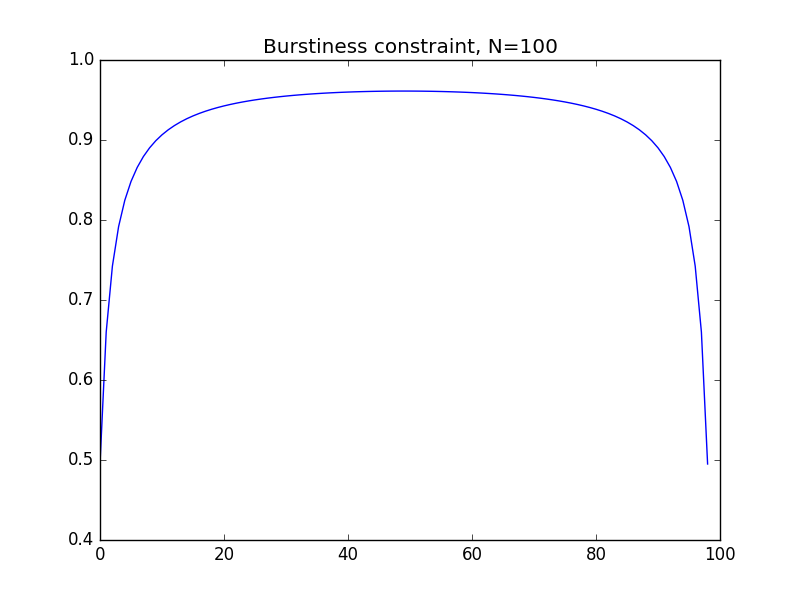
\includegraphics[scale=0.4]{img/bp}
		\caption{This plot represent the series that constraints the predictive distribution for the burstiness effect in exchangeable graph for N=100 (100 nodes)}
		\label{fig:bp}
	\end{figure}

\label{b-theorem}
\end{proof}

Interestingly this theorem tell us how the burstiness effect, for exchangeable sequence with finite capacity $N$, will collapse for a small number of observation and notably, when the number of observations get closer to the capacity.\\

A typical form of the predictive distribution $\p(y_{ij}=1 | d_i^{N,n})$ is a linear function of the sufficient statistics of the observations (see \ref{prop:diaconis}). Though the burstiness effect would have specific constraint in this case.

\begin{theorem}[Burstiness to Local Preferential Attachment] \label{th:burst_exch}
	Let $\M_g$ be a network model of a jointly exchangeable graph $G(V,E)$ such that $f_i$ and $\phi_{kk'}$ are iid for any $i$, $k$ and $k'$.Moreover,  Let $N^c$ and $N^r$ be two integer such that the the former is the number of node in a class $c$, and the second the number of node not being in $c$, such that $N^c+N^r = N$. A local degree distribution $p(d_{i,c}=n)$ of any node $i$ in $c$ is bursty iif,
	
	\begin{equation}
\Delta_n  p(y_{ij}=1 | d_{i,c}^{N,n}) \frac{\sum_{r=0}^{N_r}\dbinom{N}{n+1+r} p(d_{ir}^{N^r,r})}{\sum_{r=0}^{N_r} \dbinom{N}{n+r} p(d_{ir}^{N^r,r}) } > 0
	\end{equation}
	
	
\end{theorem}

\begin{proof}
The exchangeable graph $G(V,E)$ contains $|V|=N$ nodes. Thus in the context of the local preferential attachment we consider the degree of a node $i$, in a class $c$ containing $N_c$ nodes and we denote the degree of this node within this class by $d_{i,c}$. We note the remaining number of node by $N_r = N - N_c$. We then write  distribution of the degree inside that class by marginalizing the possible edges between $i$ and the nodes that are not in $c$. We have:
\begin{equation}
p(d_{ic}=n) = \sum_{r=0}^{N_r} p(d_{ic}=n,d_{ir}=r)
\end{equation}
From exchangeable assumptions one as:

\begin{equation}
p(d_{ic}=n) = \sum_{r=0}^{N_r} \dbinom{N}{n+r} p(d_{ic}^{N_c, n},d_{ir}^{N_r, r})
\end{equation}
Under the assumptions that each local random parameters are i.i.d, we can seperate the joint distribution: ( \textcolor{red}{on peut ouvrir la distribution avec les F et les Phi, pour voir que ca marche pour IMMSB mais pas pour ILFM, je me garde de l'écrire la pour gagner du temps !)}: 

\begin{align}
p(d_{ic}=n) &= \sum_{r=0}^{N_r} \dbinom{N}{n+r} p(d_{ic}^{N_c, n}) p(d_{ir}^{N_r, r}) \\
 &=  p(d_{ic}^{N_c, n})\sum_{r=0}^{N_r}   \dbinom{N}{n+r} p(d_{ir}^{N_r, r})
\end{align}

Finally by applying the burstiness properties as in proof \ref{proof:glob}, and product rule we can expess the burstiness in function of the predictive distribution:

\begin{equation}
b_n =  p(y_{ij}=1 | d_{i,c}^{N,n}) \frac{\sum_{r=0}^{N_r}\dbinom{N}{n+1+r} p(d_{ir}^{N^r,r})}{\sum_{r=0}^{N_r} \dbinom{N}{n+r} p(d_{ir}^{N^r,r}) }
\end{equation}

\end{proof}

\textcolor{red}{Corollaire:  avec une contrainte sur Nc et Nr, il suffit de regarder la croissance de la distribution predictive, je l'ai vue en tracant la fraction, mais je n'ai pas réussi à le prouver analytiquement ...}


%\begin{corollary}
%	A degree distribution  $p(d_i=n)$ of any node $i$ in a jointly exchangeable graph $G(V,E)$ such that it admits a predictive distribution of the form $\p(y_{ij}=1 | d_i^{N,n}) = an+b$, is bursty iff:
%Polynome solution, constraint on the positive roots, a, b > ...
%\end{corollary}

We now apply the previous results to characterize the preferential attachments effect in social networks.


\begin{proposition}
	The IMMSB models satisfy the local preferential attachments in the generative model $\M_g$.
\end{proposition}

\begin{proof}
We have:
In IMMSB one can write the predictive distribution conditioned by $d_i^{N,n}$:

\begin{equation} 
p(y_{ij} = 1 | d_i^{N,n}, \mathcal{M}) = \int_{\Theta} p(y_{ij}=1|\Theta) \frac{p(d_i^{N,n} | \Theta)}{p(d_i^{N,n})} p(\Theta) d\Theta \nonumber
\end{equation}

By only restraining the relations that occur inside class $c=\{k,k\}$, thus we note $N^c$ the total number of relations (links and non-links) in the class $c$ for node $i$, one can write the local preferential attachment:

\begin{align*} \label{eq:sum}
&p(y_{ij} = 1 | d_{ic}^{N^c,n}, \mathcal{M})  \\
&=  \frac{ \int_{\phi_{c}} p(y_{ij}=1|\phi_{c}) p(d_{ic}^{N,n} | \phi_{c}) p(\phi_{c}) d\phi_{c}}{\int_{\phi_{c}} \p(d_{ic}^{N^c,n} | \phi_{c}))       p(\phi_{c}) d\phi_{c}}   \\
&= \frac{\int_{\phi_c} \phi_c^{n+1}(1-\phi_c)^{N^c-n} \phi_c^{\lambda_1-1} (1-\phi_c)^{\lambda_0-1} d\phi_{c}}{\int_{\phi_c} \phi_c^{n}(1-\phi_c)^{N^c-n} \phi_c^{\lambda_1-1} (1-\phi_c)^{\lambda_0-1} d\phi_{c}} \\
&= \frac{ \text{B}(n+1+\lambda_1, N^c-n+\lambda_0) }{\text{B}(n+\lambda_1, N^c-n+\lambda_0)} \\
&= \frac{n+\lambda_1}{N^c + \lambda_1 +\lambda_0}
\end{align*}

Where $\text{B}()$ is the beta function. The last equation show that the predictive likelihood is strictly crescent with $n$.

\end{proof}

\begin{proposition}
	The ILFM models statisfy the local preferential attachments. in the generative mode $\M_g$.
\end{proposition}
\begin{proof}
	\textcolor{red}{This is not sure actually, local proof for ILFM to finish...}
\end{proof}

\begin{proposition}
	The ILFM and IMMSB models do not satisfy the global and local preferential attachments. in the mode $\M_e$.
\end{proposition}

The proof of this statement is trivially true in the sens that given $\mat{F}$ and $\mat{\Theta}$, the link likelihood is fully determined and hence do not depend on new links being generated. Furthermore, we show empirical counter example, where figure \ref{fig:gen_burst_mmsb} show some complex pattern in the empirical distribution of the overall degree that are clearly non bursty.

\begin{proposition} \label{prop:diaconis}
	Both ILFM and IMMSB models satisfy the feature burstiness for $n < L$ under some conditions on their hyperparameters  and $L$ a number of observation depending of the hyperparameters.
\end{proposition}

\begin{proof}
The Diaconis-Ilvisaker theorem \cite{diaconis1979conjugate} state \emph{'subject to regularity conditions, the conjugate priors typically used satisfy, and are characterized by, a  similar relation of posterior linearity'}:
\begin{equation}
\E_\Theta[\E_{X|\Theta}[X\mid \Theta] \mid X=x] = ax+b \quad \text{for} \quad x=0,1,2,... \nonumber
\end{equation}

Especially, the Dirichlet Process and the Indian Buffet Process, as prior for the latent features, are typically build on the suitable conjugate distribution respectively Dirichlet-Multinomial and Beta-Bernoulli. Furthermore, this claim is highlighted by the Gibbs update that corroborate the feature burstiness effect:
\begin{align} \label{eq:feat_up}
&\p(f_{ik} = 1 | F^{-ik}) = \frac{m_k^{-ik}}{N} \qquad \text{ILFM feature update} \nonumber \\
&\p(f_{ik} = 1 | F^{-ik}) = \frac{n_{ik}^{-z_{ij}}+\alpha_k}{N+\alpha_.} \qquad \text{IMMSB feature update} \nonumber \\
\end{align}

Where the $m_k^{-ik}$ described the number of elements that have the $k$-iem feature active except for element $i$, similarly $n_{ik}^{-z_{ij}}$ represents the number of times that $i$ was assigned to $k$ except for relation $(ij)$ (class membersehip are jointly sampled in MMSB).

By applying theorem \ref{th:burst_exch} for linear predictive distribution, it can be easily show that the burstiness is true below a number $L$ which is the positive roots of the following polynoms:
\begin{equation}
	 an^2 + 3an - a(N-1) + b(N+1) = 0
\end{equation}

The condition on the hyperparameters $a$ and $b$ arise in order to find a stricly positive roots of this polynom. In the case of ILFM and IMMSB, it is equivalent to solve the polynom whith a=1 and  $b=0$ or $b=\alpha_k$ for respectively ILFM and IMMSB. The positive roots arise in this case if $b < 1$, which determines $L$.
\end{proof}

We represent tree networks generated by ILFM in figure \ref{fig:gen_burst_ilfm} and IMMSB \ref{fig:gen_burst_mmsb}. We compute a goodness of fit to quantify the power law hypothesis on the empirical degree distributions. The protocol is described in section \ref{sec:experiments-busrt}. As an empirical illustration for our claims on preferential attachment, we show a 3*3 figure where each columns is particular setting of hyper-parameter and the rows are respectively, the global degree distribution, the local degree distribution and feature distribution (on a max a assignment point of view).

As we can see in the experiments, we can generate networks that do not fit the burstiness definition on the overall degree distribution.

\begin{figure}[h]
	\centering
	
	\minipage{0.16\textwidth}
	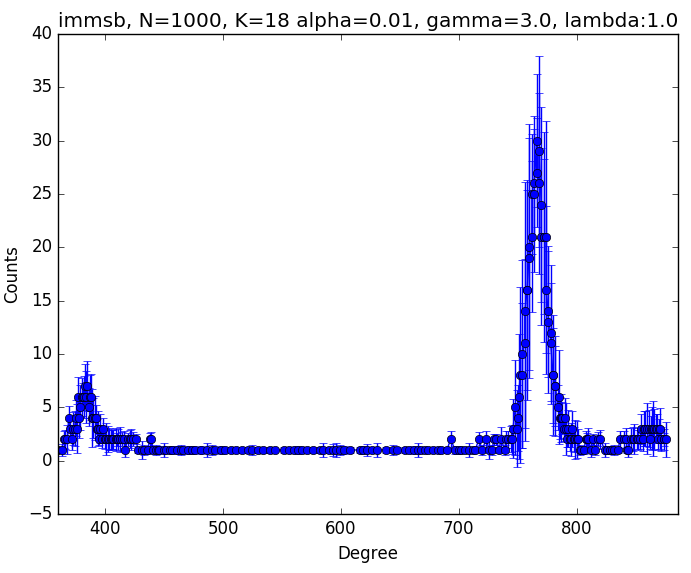
\includegraphics[width=3.2cm, height=3.7cm]{img/M_g_peaks/figure_1}
	\endminipage
		\minipage{0.16\textwidth}
	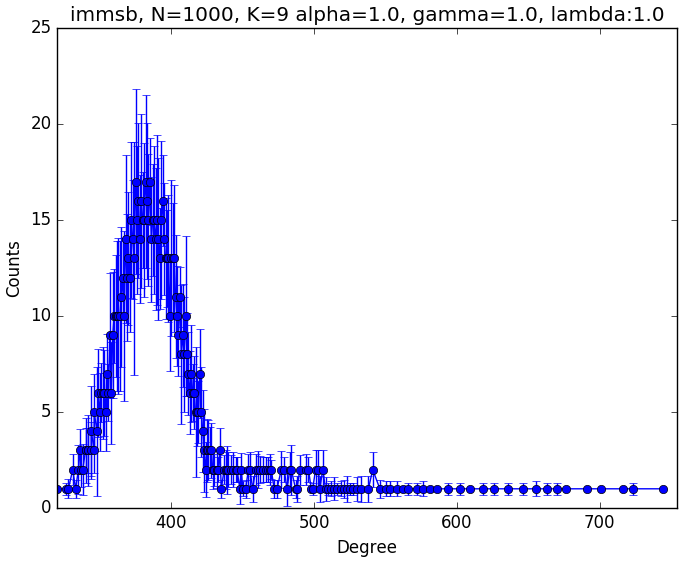
\includegraphics[width=3.2cm, height=3.7cm]{img/M_g_power_law/figure_1}
	\endminipage
	\minipage{0.16\textwidth}
	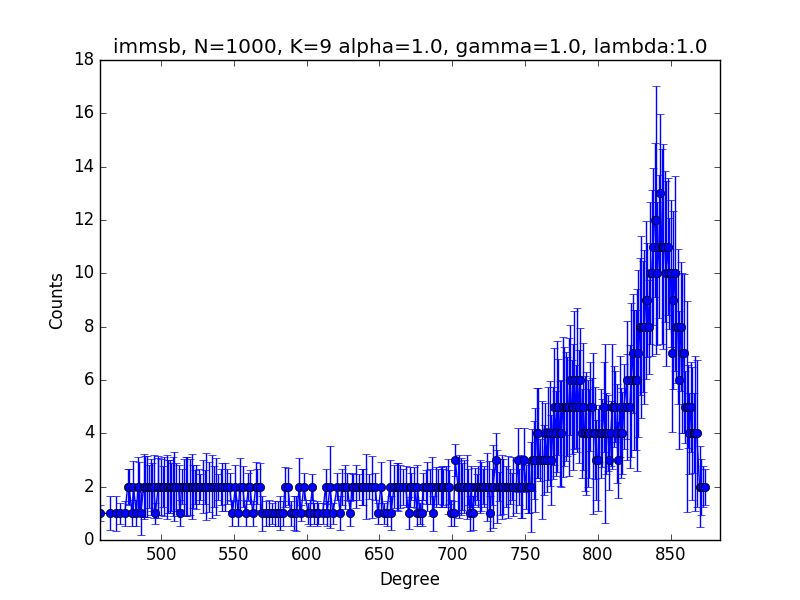
\includegraphics[width=3.2cm, height=3.7cm]{img/M_g_regular/figure_1}
	\endminipage
		\vspace{-0.4cm}
	\minipage{0.16\textwidth}
	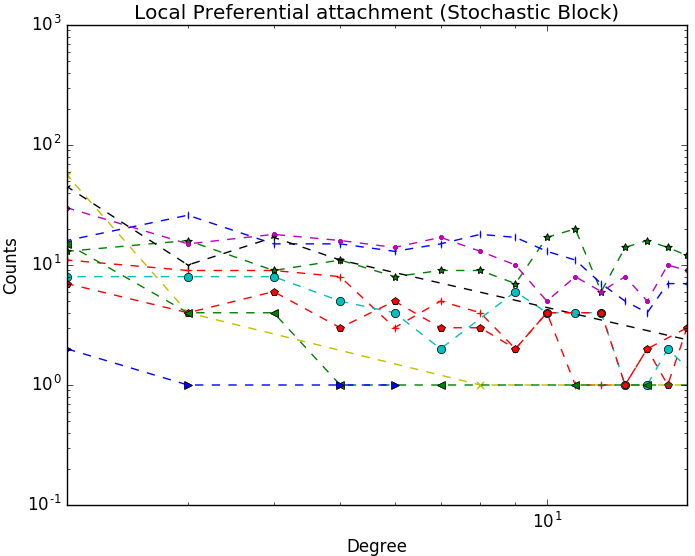
\includegraphics[width=3.2cm, height=3.7cm]{img/M_g_peaks/figure_3}
	\endminipage
		\minipage{0.16\textwidth}
	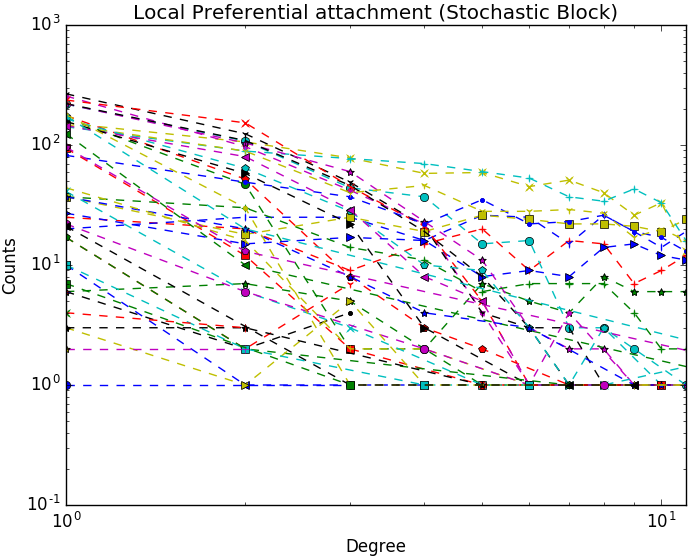
\includegraphics[width=3.2cm, height=3.7cm]{img/M_g_power_law/figure_3} 
	\endminipage
	\minipage{0.16\textwidth}
	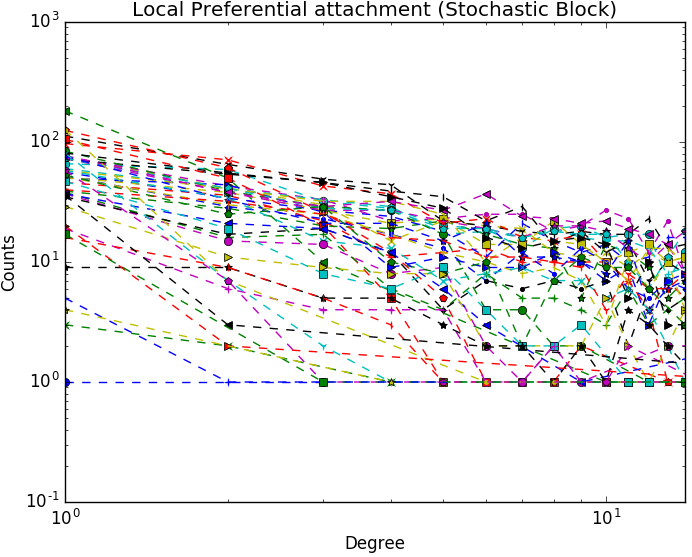
\includegraphics[width=3.2cm, height=3.7cm]{img/M_g_regular/figure_3}
	\endminipage
		\vspace{-0.4cm}
	\minipage{0.16\textwidth}
	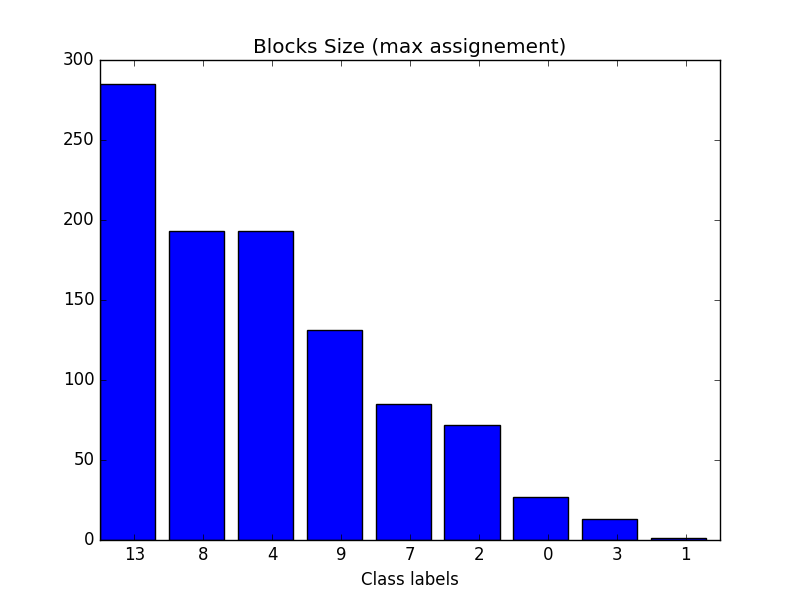
\includegraphics[width=3.2cm, height=3.7cm]{img/M_g_peaks/figure_5}
	\endminipage
	\minipage{0.16\textwidth}
	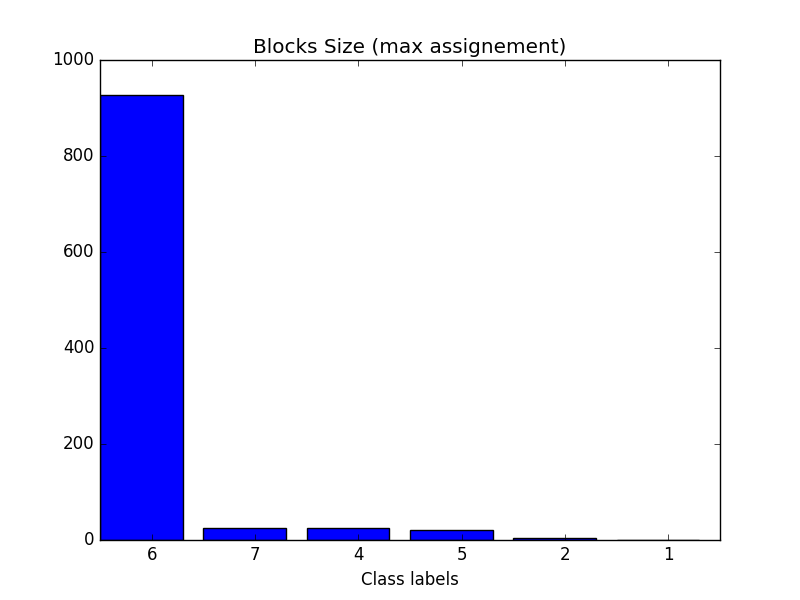
\includegraphics[width=3.2cm, height=3.7cm]{img/M_g_power_law/figure_5} 
	\endminipage
	\minipage{0.16\textwidth}
	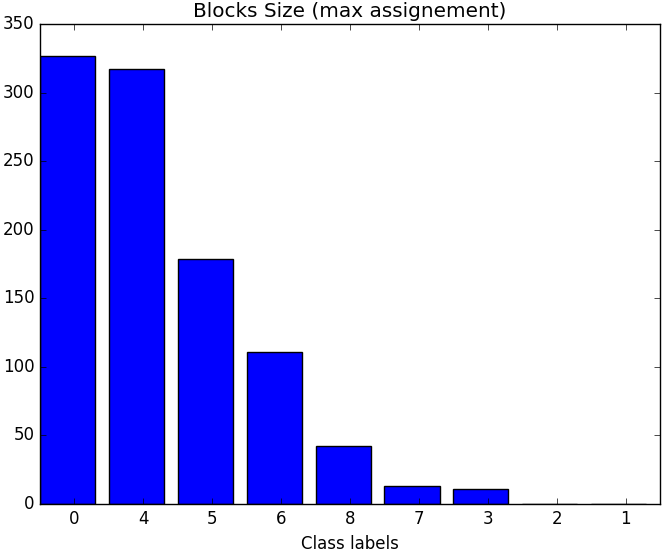
\includegraphics[width=3.2cm, height=3.7cm]{img/M_g_regular/figure_5}
	\endminipage
	\caption{Generated Networks with in three different settings (same set than for figure \ref{fig:gen_blocks}). The upper figures show the global preferentual attachment. The lower figures show the local preferential attachment. While global preferential attachment is not a pure features of model, we see that the local preferential attachment has linear form in the log-log space.}
	\label{fig:gen_burst_mmsb}
\end{figure}



